
%%%%%%%%%%%%%%%%%%%%%%%InSTA2015の論文
\chapter{I/O テストデータパターンを使ったテストケース抽出手法}\label{chap:4}
本章では,テスト分析において,テスト条件を網羅的に特定する方法として,テスト実行時のデータの入出力(以降I/Oと呼ぶ)に着目する.
テストベースを分析する際に,テスト実行時のI/Oの要素で分解し網羅性を確認する方法を提案する.
3章の題材を使って提案手法の適用評価を行う.
また,現実の開発プロジェクトのテストケースと提案手法で特定したテスト条件の内容を比較し,手法を適用することで見つけることができるテスト条件にどのようなものがあるかを確認する.

\newpage
\section{研究の概要} \label{sec:4-1}
\subsection{研究の目的} \label{sec:4-1-1}
3章の実験を通して,テストカテゴリベースドテストの適用に一定の効果は確認できたものの,
知識を与えても期待した数のテスト条件を特的できるわけではないことがわかった.
また,業務経歴3年未満の技術者には有効であったが,3年以上の技術者にはあまり効果がないこともわかった.
テストカテゴリベースドテストは,テストベースの分析に論理的機能構造をガイドとして使用することを明示しているだけであり,具体的な分析手順について定義できていない.
本章では,テスト条件を網羅的に特定する方法として,テスト実行時のデータのI/Oに着目する方法を提案する.
提案する手法が適用可能であることを評価し,手法を適用することにって適用前では特定できなかったテスト条件が
特定できるようになることを現実のプロジェクトのテストケースとの比較で評価する,

\subsection{I/Oテストデータパターン} \label{sec:4-1-1}
テストを実行するためには,データをテスト対象となる$AS$のタスク群$Ta$に対して,源泉$So$から入力$In$し,$Ta$から$So$への出力$Out$による実際の結果と期待結果とで比較する.

たとえば,シンプルな機能の四則演算の計算結果が正しいことを検証するときには,$AS$の外部となる源泉$So$から複数の値を入力$In$し,タスク群$Ta$がそれらの値を計算し,計算結果をテスト対象の外部である$So$へ出力$Out$する.

これは図~\ref{fig:D-3-Fig4}で示している「外部からのデータ入力,外部へのデータ出力」というパターンになる.また,$So$から$In$する数値に対して,保持データ$Ds$である固定比率を使って計算を行う場合,$Ta$は$Ds$から適切な比率を呼び出し,計算にその値を利用してから計算結果を$So$へ$Out$する.
これは図~\ref{fig:D-3-Fig4}で示している例「外部と内部からのデータ入力,外部へのデータ出力」となる.
\begin{figure}[htbp]
 \begin{center}
 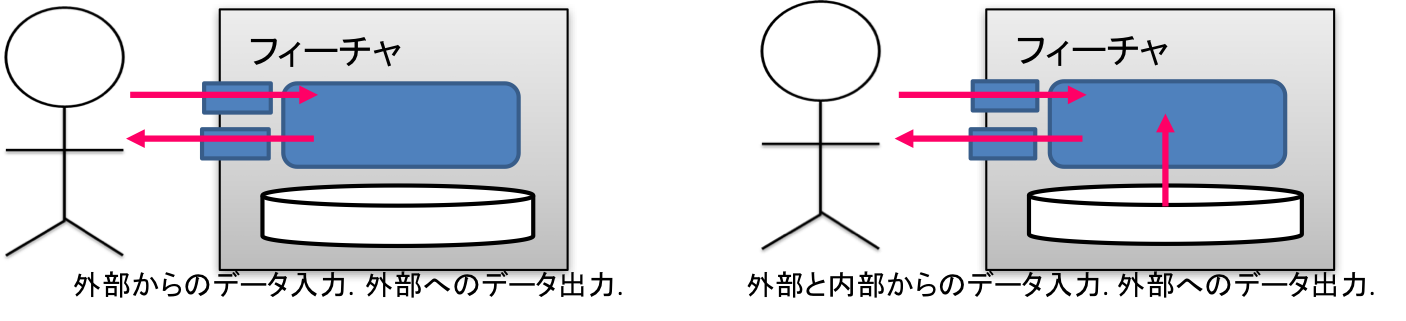
\includegraphics[width=12cm]{./image/D-3-Fig4.png}
 \caption{テスト対象へのデータ入出力の説明}
 \label{fig:D-3-Fig4}
 \end{center}
\end{figure}

テスト実行をするときの$Ta$へのデータを$In$する方法は,外部からの入力,内部に保持したデータの入力,外部と内部からの入力の3パターンに分類できる.
同じようにテスト対象からのアウトプット方法は外部への出力,内部に保持したデータの出力,外部と内部からデータの出力の3パターンに分類できる.
これらテスト対象に対するテスト実行時のデータの入出力をまとめたパターンは図~\ref{fig:D-4-Fig6}のように9パターンに集約できる.

\begin{figure}[htbp]
\begin{center}
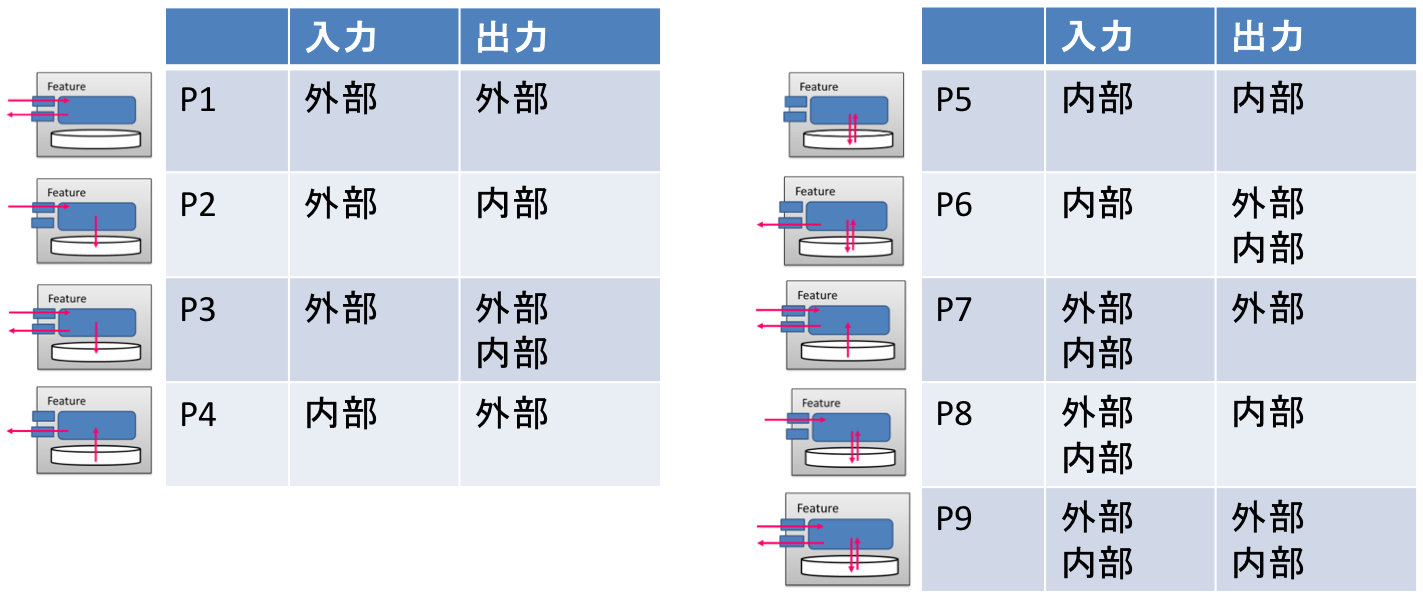
\includegraphics[width=14cm]{./image/D-3-Fig5.png}
\caption{I/Oテストデータパターン}
\label{fig:D-4-Fig6}
\end{center}
\end{figure}

これをI/Oテストデータパターンと呼ぶ.
I/Oテストデータパターンがテスト実行時のデータの入出力から見た全体集合となる.

Whittakerによって提案されているフォールトモデル\cite{whittaker2003break}は,$AS$の$Ta$に対する$In$と$Out$のモデルに関する類似の研究である.フォールトモデルの目的はフォールトを見つけることであり,I/Oテストデータパターンで提示しているデータの入出力モデルはテストベースからテスト条件の中の仕様項目を特定するためのモデルとして使われる.


注意すべきこととしてI/Oテストデータパターンはテスト対象の外部からの観察が可能なものを選ぶことがあげられる.
$Ta$の起動終了に使われる内部のコマンド(シグナルやイベント)は,データパターンへ分類をするときに考慮しない.
なぜならこの手法はブラックボックステストのためのテストベースの分析手法であり,$AS$内部のシグナルやイベントのような外部観察ができないコマンドは,システムテストレベルでのブラックボックステストでは,明示的に考慮できないからである.

テスト分析で特定した仕様項目は,テスト実行をした際の入出力にて確認することができなければならないので,すべてが9パターンのどれかに分類できると考えられる.

\subsection{I/Oテストデータパターンの適用評価}

P1からP9のI/Oテストデータパターンは,単一の入出力の全体像となる.
$So$からデータの$In$を行い,$So$へ$Out$する間に,テスト対象となる$Ta$を推定した論理的機能構造の入力調整,出力調整,変換,貯蔵を通過する.
I/OテストデータパターンのP1からP9のそれぞれが論理的機能構造のどの要素に該当するかを表~\ref{tbl:D-4-tbl1}にまとめた.

% Table generated by Excel2LaTeX from sheet 'Sheet3'
\begin{table}[htbp]
  \centering
  \caption{I/Oテストデータパターンと論理的機能構造}
    \begin{tabular}{|r|p{4em}|l|l|l|p{4em}|l|l|}
    \hline
          & \multicolumn{1}{l|}{} & \multicolumn{1}{p{4em}|}{\textbf{入力調整}} & \multicolumn{1}{p{4em}|}{\textbf{出力調整}} & \multicolumn{1}{p{4em}|}{\textbf{変換}} & \textbf{貯蔵} & \multicolumn{1}{p{2em}|}{\textbf{サポート}} & \multicolumn{1}{p{1.915em}|}{\textbf{相互作用}} \bigstrut\\
    \hline
    \multicolumn{1}{|p{1.5em}|}{\textbf{入力}} & \textbf{外部} & \multicolumn{1}{p{4em}|}{P1,P2,P3} &       & \multicolumn{1}{p{4em}|}{P1,P2,P3} & \multicolumn{1}{l|}{} &       &  \bigstrut\\
\cline{2-8}          & \textbf{内部} &       &       & \multicolumn{1}{p{4em}|}{P4,P5,P6} & P4,P5,P6 &       &  \bigstrut\\
\cline{2-8}          & \textbf{外部と内部} & \multicolumn{1}{p{4em}|}{P7,P8,P9} &       & \multicolumn{1}{p{4em}|}{P7,P8,P9} & P7,P8,P9 &       &  \bigstrut\\
    \hline
    \multicolumn{1}{|p{1.5em}|}{\textbf{出力}} & \textbf{外部} &       & \multicolumn{1}{p{4em}|}{P1,P4,P7} &       & \multicolumn{1}{l|}{} &       &  \bigstrut\\
\cline{2-8}          & \textbf{内部} &       &       &       & P2,P5,P8 &       &  \bigstrut\\
\cline{2-8}          & \textbf{外部と内部} &       & P3,P6,P9 &       & P3,P6,P9 &       &  \bigstrut\\
    \hline
    \end{tabular}%
  \label{tbl:D-4-tbl1}%
\end{table}%


P1に分類できるシンプルな四則演算を行う$Ta$の場合,外部からの入力に対して外部に出力する間に,
図~\ref{fig:D-4-Fig7}のように論理的機能構造の入力調整,変換,出力調整を通過する.
そのため,P1は,表~\ref{tbl:D-4-tbl1}の以下の3箇所にプロットされている.
\begin{itemize}
  \item 列:入力調整 行:入力/外部
  \item 列:出力調整 行:出力/外部
  \item 列:変換 行:入力/外部
\end{itemize}

このデータフローで通過する3箇所が,P1の場合の期待結果を確認する候補となる.
これらを本研究ではチェックポイントと呼ぶ.
チェックポイントのうち,期待結果を意図的に確認する必要があると判断したものがテスト分析で特定すべき仕様項目,つまりテスト条件となる.

 \begin{figure}[htbp]
 \begin{center}
 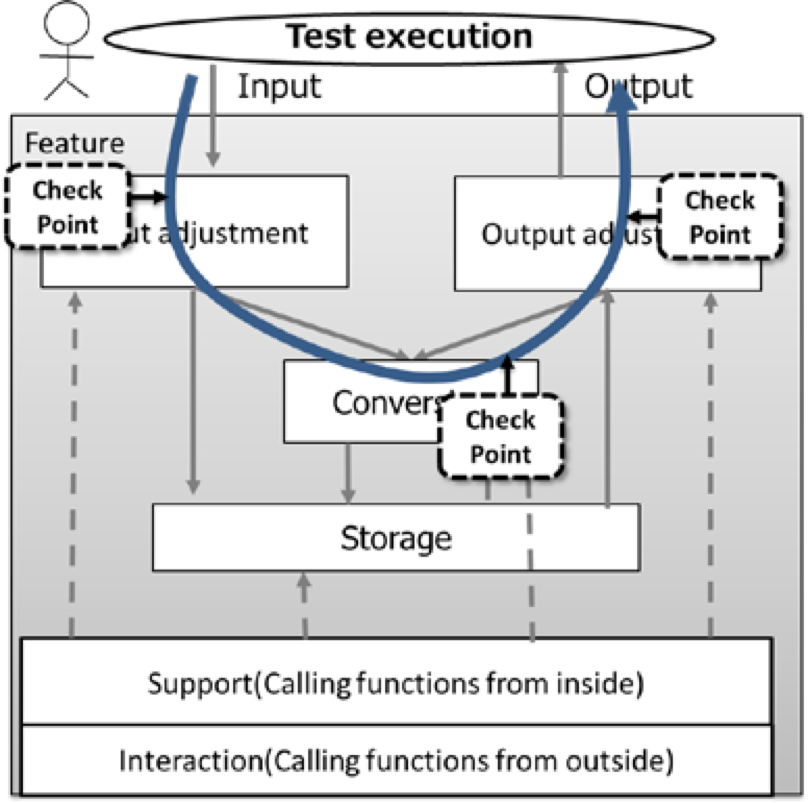
\includegraphics[width=10cm]{./image/D-4-Fig7.png}
 \caption{I/Oテストデータパターンのデータの流れ}
 \label{fig:D-4-Fig7}
 \end{center}
 \end{figure}

データフローの中で通過する3箇所のチェックポイントのうち,少なくとも1つのチェックポイントをテスト条件として特定するが,全てが実際に期待結果を確認する仕様項目になるとは限らない.
例えば,テストすべき仕様項目を特定する際に,入力調整に該当する入力の際に適切な値だけ受け入れることと,変換に該当する計算が適切に行われていることはテストすべきであるが,出力調整が適切にされることは,すでに自明であるためにテストケースとする必要がないということが考えられるためである.

また,表~\ref{tbl:D-4-tbl1}では,サポートと相互作用についてはデータパターンがプロットされていない.
論理的機能構造の要素である入力調整,出力調整,変換,貯蔵は,外部観察可能な単一の入出力のみを考慮している分類であるのに対して,サポートと相互作用は,単一の入出力だけではなく,関係する他の処理の呼び出しに着目して仕様項目を特定するための分類であり,P1からP9のI/Oテストデータパターンは単一の入出力の全体像だからである.

サポートと相互作用に分類される仕様項目は,呼び出した後の出力で期待結果を確認する.
呼び出された機能のI/Oテストデータパターンは,論理的に全パターンが発生する可能性がある.


\newpage
\section{これまでの実験結果を使った調査}
本節では,I/Oテストデータパターンの考え方を3章で行なった被験者を使ってテストカテゴリを使った分析手法の習得前と習得後を比較する実験の結果による適用評価を行う.
演習にて利用したテスト分析の講師解答例をI/Oテストデータパターンに分類するために,P1からP9の識別子を解答例の仕様項目の属性として付与し,「3.2節 グループ単位の検証実験からの考察」での実験結果を3章の表~\ref{tbl:D-3-tbl4}で示した評価レベルのアプローチをベースに整理する.

その後,表~\ref{tbl:D-4-tbl1}と同じフォーマットの表に出現結果を当てはめて,これらの題材にてどのI/Oテストデータパターンが現れるのかを調査した.

\subsection{論理的機能構造の適用評価の分析}
「グループ単位の検証実験からの考察」では,ヘッドセットのフィーチャであるボリュームコントロールと,フライト予約システムのフィーチャである新規フライト予約の2種類の異なった$AS$を実験に使用した.
被験者のグループがテスト分析手法の知識を得ることでテスト条件をどのように多く特定できるようになるかを実験している.
この実験結果をI/Oテストデータパターンにて評価した結果は,表~\ref{tbl:D-4-tbl7}と表~\ref{tbl:D-4-tbl8}に示したとおりである.
前節の結果と本節の結果では行数が異なる理由は, 仕様項目のいくつかは同じテストカテゴリに属する仕様項目でも異なったI/Oデータパターンを付与している場合があり,そのためテストカテゴリを論理的昨日構造とは違う分類をしているためである.
表~\ref{tbl:D-4-tbl7}と表~\ref{tbl:D-4-tbl8}が示すとおり, P1, P2, P4, P7 が検証実験で使ったフィーチャセットに対応するI/Oテストデータパターンとなる.

% Table generated by Excel2LaTeX from sheet 'データの入出力ごとフェリカ (掲載用加工)'
\begin{table}[htbp]
  \centering
\caption{音楽再生機器の演習結果とI/Oテストデータパターン}
    \begin{tabular}{|l|l|l|l|l|l|l|l|}
    \hline
    \multicolumn{2}{|c|}{\multirow{2}[4]{*}{論理的機能構造}} & \multicolumn{6}{c|}{チーム} \bigstrut\\
\cline{3-8}    \multicolumn{2}{|c|}{} & TM1   & TM2   & TM3   & TM4   & TM5   & TM6 \bigstrut\\
    \hline
    \textbf{変換} & P4    & B     & B     & B     & B     & -     & B \bigstrut\\
    \hline
    \textbf{変換} & P1    & B     & A${}^\text{+}$    & B     & B     & B     & - \bigstrut\\
    \hline
    \textbf{出力} & P7    & -     & -     & -     & -     & -     & A${}^\text{+}$ \bigstrut\\
    \hline
    \textbf{貯蔵} & P2    & -     & A${}^\text{+}$    & -     & A${}^\text{+}$    & A${}^\text{+}$    & - \bigstrut\\
    \hline
    \textbf{サポート} & P1    & B     & B     & B     & B     & B     & B \bigstrut\\
    \hline
    \textbf{相互作用} & P1    & B     & A${}^\text{+}$    & A${}^\text{+}$    & A${}^\text{+}$    & A${}^\text{+}$    & A${}^\text{+}$ \bigstrut\\
    \hline
    \textbf{相互作用} & P4    & B     & B     & B     & A${}^\text{+}$    & B     & A${}^\text{+}$ \bigstrut\\
    \hline
    \end{tabular}%
\label{tbl:D-4-tbl7}%
\end{table}%

% Table generated by Excel2LaTeX from sheet 'D論4章用'
\begin{table}[htbp]
  \centering
\caption{フライト予約システムの演習結果とI/Oテストデータパターン}
    \begin{tabular}{|l|l|l|l|}
    \hline
    \multicolumn{2}{|c|}{\multirow{2}[4]{*}{論理的機能構造}} & \multicolumn{2}{c|}{チーム} \bigstrut\\
\cline{3-4}    \multicolumn{2}{|c|}{} & TM1   & TM2 \bigstrut\\
    \hline
    \textbf{変換} & P7    & A     & A \bigstrut\\
    \hline
    \textbf{入力} & P1    & B     & B \bigstrut\\
    \hline
    \textbf{入力} & P7    & A     & - \bigstrut\\
    \hline
    \textbf{入力} & P4    & -     & - \bigstrut\\
    \hline
    \textbf{出力} & P4    & B     & B \bigstrut\\
    \hline
    \textbf{出力} & P4    & A     & A \bigstrut\\
    \hline
    \textbf{出力} & P7    & B     & B \bigstrut\\
    \hline
    \textbf{貯蔵} & P2    & A${}^\text{+}$    & A${}^\text{+}$ \bigstrut\\
    \hline
    \textbf{貯蔵} & P7    & A     & A \bigstrut\\
    \hline
    \textbf{サポート} & P1    & -     & A${}^\text{+}$ \bigstrut\\
    \hline
    \textbf{サポート} & P1    & B     & B \bigstrut\\
    \hline
    \textbf{相互作用} & P4    & B     & A \bigstrut\\
    \hline
    \end{tabular}%
\label{tbl:D-4-tbl8}%
\end{table}%

I/Oテストデータパターンで評価レベルの数を集約した結果が表~\ref{tbl:D-4-tbl9}と表~\ref{tbl:D-4-tbl20}である.
各I/Oテストデータパターンにて A と A${}^\text{+}$ の割合を確認すると,P2のみが音楽再生機器,フライト予約システムの両方の検証実験で100%となっているため,P2のデータパターンに対する効果が最も高いと言える.

音楽再生機器の場合,P2に分類された仕様項目は「ボリューム値の保存」である.
この仕様項目はテストベースに記述はされているものの,ボリュームコントロールのセクションとは別のセクションに記述されている.
飛行機予約システムの場合,P2に分類された仕様項目は注文内容の「データベースへの保存」である.
データベースへの保存に関して,テストベースには,詳しい記載は無い.
これらの観察結果は2章にて述べたテスト条件の特定を困難にしている課題の一つである「明白に必要だと思われる仕様の一部分が記述されていない.」と一致する.

% Table generated by Excel2LaTeX from sheet 'D論4章用'
\begin{table}[htbp]
  \centering
  \caption{I/Oテストデータパターンごとの集計結果}
    \begin{tabular}{lllllr}
    音楽再生機器 &       &       &       &       &  \bigstrut[b]\\
    \hline
    \multicolumn{1}{|c|}{\multirow{2}[4]{*}{I/O パターン}} & \multicolumn{4}{c|}{評価レベル}    & \multicolumn{1}{c|}{\multirow{2}[4]{*}{割合}} \bigstrut\\
\cline{2-5}    \multicolumn{1}{|c|}{} & \multicolumn{1}{l|}{A${}^\text{+}$} & \multicolumn{1}{l|}{A} & \multicolumn{1}{l|}{-} & \multicolumn{1}{l|}{B} & \multicolumn{1}{c|}{} \bigstrut\\
    \hline
    \multicolumn{1}{|l|}{P1} & \multicolumn{1}{r|}{6} & \multicolumn{1}{r|}{0} & \multicolumn{1}{r|}{7} & \multicolumn{1}{r|}{11} & \multicolumn{1}{r|}{35.3\%} \bigstrut\\
    \hline
    \multicolumn{1}{|l|}{P2} & \multicolumn{1}{r|}{3} & \multicolumn{1}{r|}{0} & \multicolumn{1}{r|}{3} & \multicolumn{1}{r|}{0} & \multicolumn{1}{r|}{100.0\%} \bigstrut\\
    \hline
    \multicolumn{1}{|l|}{P4} & \multicolumn{1}{r|}{2} & \multicolumn{1}{r|}{0} & \multicolumn{1}{r|}{1} & \multicolumn{1}{r|}{9} & \multicolumn{1}{r|}{18.2\%} \bigstrut\\
    \hline
    \multicolumn{1}{|l|}{P7} & \multicolumn{1}{r|}{1} & \multicolumn{1}{r|}{0} & \multicolumn{1}{r|}{5} & \multicolumn{1}{r|}{0} & \multicolumn{1}{r|}{100.0\%} \bigstrut\\
    \hline
    \multicolumn{5}{l}{割合 = (A${}^\text{+}$  +  A) /(A${}^\text{+}$  +  A + B) } &  \bigstrut[t]\\
    \end{tabular}%
\label{tbl:D-4-tbl9}%
\end{table}%

% Table generated by Excel2LaTeX from sheet 'D論4章用'
\begin{table}[htbp]
  \centering
  \caption{I/Oテストデータパターンごとの集計結果}
    \begin{tabular}{lllllr}
    フライト予約 &       &       &       &       &  \bigstrut[b]\\
    \hline
    \multicolumn{1}{|c|}{\multirow{2}[4]{*}{I/O パターン}} & \multicolumn{4}{c|}{評価レベル}    & \multicolumn{1}{c|}{\multirow{2}[4]{*}{}} \bigstrut\\
\cline{2-5}    \multicolumn{1}{|c|}{} & \multicolumn{1}{l|}{A${}^\text{+}$} & \multicolumn{1}{l|}{A} & \multicolumn{1}{l|}{-} & \multicolumn{1}{l|}{B} & \multicolumn{1}{c|}{} \bigstrut\\
    \hline
    \multicolumn{1}{|l|}{P1} & \multicolumn{1}{r|}{1} & \multicolumn{1}{r|}{0} & \multicolumn{1}{r|}{1} & \multicolumn{1}{r|}{4} & \multicolumn{1}{r|}{20.0\%} \bigstrut\\
    \hline
    \multicolumn{1}{|l|}{P2} & \multicolumn{1}{r|}{2} & \multicolumn{1}{r|}{0} & \multicolumn{1}{r|}{0} & \multicolumn{1}{r|}{0} & \multicolumn{1}{r|}{100.0\%} \bigstrut\\
    \hline
    \multicolumn{1}{|l|}{P4} & \multicolumn{1}{r|}{0} & \multicolumn{1}{r|}{3} & \multicolumn{1}{r|}{2} & \multicolumn{1}{r|}{3} & \multicolumn{1}{r|}{50.0\%} \bigstrut\\
    \hline
    \multicolumn{1}{|l|}{P7} & \multicolumn{1}{r|}{0} & \multicolumn{1}{r|}{3} & \multicolumn{1}{r|}{1} & \multicolumn{1}{r|}{2} & \multicolumn{1}{r|}{60.0\%} \bigstrut\\
    \hline
    \multicolumn{5}{l}{割合 = (A${}^\text{+}$  +  A) /(A${}^\text{+}$  +  A + B) } &  \bigstrut[t]\\
    \end{tabular}%
\label{tbl:D-4-tbl20}%
\end{table}%

\subsection{I/Oテストデータパターンの出現傾向の調査}

実験にて利用した2つの演習題材に対するテスト分析の講師解答例をI/Oテストデータパターンに分類した結果が表~\ref{tab:addlabel-3}である.
表~\ref{tab:addlabel-3}の結果からわかるとおり,この実験の題材にて使われたI/Oテストデータパターンは,P1とP2とP4とP7の4つであった.
またP1でプロットされているのは入力調整と変換のみであり,出力調整に該当するテスト条件は無かった.
同様にP2は貯蔵のみ,P4は変換と出力調整のみであり,各I/Oテストデータパターンでは,テスト実行のデータフローの中で期待結果を確認するチェックポイントが限られていることが確認できた.

% Table generated by Excel2LaTeX from sheet 'Sheet3'
\begin{table}[htbp]
  \centering
  \caption{I/Oテストデータパターンの出現傾向の調査結果}
    \begin{tabular}{|r|p{4em}|p{4em}|p{4em}|p{3em}|p{3em}|p{4em}|p{4em}|}
    \hline
          & \multicolumn{1}{l|}{} & \multicolumn{1}{p{4em}|}{\textbf{入力調整}} & \multicolumn{1}{p{4em}|}{\textbf{出力調整}} & \multicolumn{1}{p{4em}|}{\textbf{変換}} & \multicolumn{1}{p{4em}|}{\textbf{貯蔵}} & \multicolumn{1}{p{2em}|}{\textbf{サポート}} & \multicolumn{1}{p{1.915em}|}{\textbf{相互作用}} \bigstrut\\
    \hline
    \multicolumn{1}{|p{1.5em}|}{\textbf{入力}} & \textbf{外部} & P1(F) &       & P1(V) &       &       &  \bigstrut\\
\cline{2-8}          & \textbf{内部} &       &       & P4(V) &       &       &  \bigstrut\\
\cline{2-8}          & \textbf{外部と内部} & \multicolumn{1}{p{4em}|}{P7(F)} &       & \multicolumn{1}{p{4em}|}{P7(F)} & \multicolumn{1}{p{4em}|}{P7(F)} &       &  \bigstrut\\
    \hline
    \multicolumn{1}{|p{1.5em}|}{\textbf{出力}} & \textbf{外部} &       & P4(F)とP7(VF) &       &       & P1(V) & \multicolumn{1}{|p{3em}|}{P1(V), P4(VF)} \bigstrut\\
\cline{2-8}          & \textbf{内部} &       &       &       & \multicolumn{1}{p{4em}|}{P2(VF)} & P2(F) &  \bigstrut\\
\cline{2-8}\cline{8-8}          & \textbf{外部と内部} &       &       &       &       &       &  \bigstrut\\
    \hline
    \end{tabular}%
  \label{tab:addlabel-3}%
\end{table}%

\subsection{サポートと相互作用に関する考察}
前述したように,論理的機能構造の要素の中で,サポートと相互作用は,単一の$Ta$に対するデータの入出力だけではなく,関係する他の$Ta$の呼び出しに着目している.
テスト条件として特定するのは,最初のテストアクションで操作されるタスク$Ta_i$の入出力のデータフローのチェックポイントからではなく,他のタスク$Ta_j$の入出力のデータフローのチェックポイントである.

表~\ref{tbl:D-4-tbl1}では,サポートと相互作用に分類できるI/Oテストデータパターンを特定できていなかったが,実際のテスト分析結果から調査した結果,表~\ref{tab:addlabel-3}で示したとおり,P1とP2とP4とP7にテスト条件を分類した.

表~\ref{tab:D-4-SandI}は,表~\ref{tab:addlabel-3}にてサポートと相互作用に分類したテスト条件の一覧である.

% Table generated by Excel2LaTeX from sheet 'Sheet3'
\begin{table}[htbp]
  \centering
  \caption{サポートと相互作用に分類されたテスト条件一覧}
    \begin{tabular}{|r|p{8em}|p{4em}|p{4em}|p{5em}|}
    \hline
    \multicolumn{1}{|p{4em}|}{\textbf{フィーチャ}} & \textbf{テスト条件} & \textbf{I/Oテストデータパターン} & \textbf{呼び出し} & \textbf{論理的機能構造} \bigstrut\\
    \hline
    \multicolumn{1}{|p{4em}|}{\textbf{ボリュームコントロール}} & 再生中,通話中以外音量値の調節を無視する & P1    & 割り込み  & サポート \bigstrut\\
\cline{2-5}          & 通話と再生の音量値を調節しても互いに影響を受けない & P1    & リソース共有 & 相互作用 \bigstrut\\
\cline{2-5}          & リセットで音量値がデフォルト値に戻る & P4    & リソース共有 & 相互作用 \bigstrut\\
    \hline
    \multicolumn{1}{|p{4em}|}{\textbf{新規フライト予約}} & 「既存注文検索」へ注文が反映すること & P4    & 他への反映 & 相互作用 \bigstrut\\
\cline{2-5}          & 「注文件数グラフ」へ注文が反映すること & P4    & 他への反映 & 相互作用 \bigstrut\\
\cline{2-5}          & 「注文履歴」へ注文が反映すること & P4    & 他への反映 & 相互作用 \bigstrut\\
\cline{2-5}          & 登録時にチケット在庫なしの場合エラーになること & P1    & 他処理連動 & サポート \bigstrut\\
\cline{2-5}          & 注文挿入中に強制終了すると処理をロールバックすること & P2    & 他処理連動 & サポート \bigstrut\\
    \hline
    \end{tabular}%
  \label{tab:D-4-SandI}%
\end{table}%

サポートと相互作用として特定する仕様項目の傾向について以下のような考察が出来る.
サポートに分類されるテスト条件として特定するのは,フィーチャセットでのテスト実行時のアクションによって操作されるタスク$Ta_i$から内部的に連動して呼び出される別のタスク$Ta_j$のチェックポイントをテスト条件とすべき仕様項目として特定する場合である.

この例では,全てテスト対象の$Ta_i$へのデータ入力に対して$Ta_j$の結果を出力するだけであるため,I/OテストデータパターンはP1としている.

一方,相互作用は,テスト実行時に,テスト対象の$Ta_i$へのテストアクションによるデータ入力による副作用を確認する.副作用が起きる例としては,入力データを$Ds$へ登録した際の状態の変化などが挙げられる.
この確認をするためには,他フィーチャセットの$Ta_j$に対するテストアクションを行い,$Ta_j$に対するデータフローのチェックポイントをテスト条件とすべき仕様項目として特定する場合である.

音楽再生機器のボリュームコントロールにて特定した2つの仕様項目は,$Ta_i$へのテストアクションを行なった後に,その副作用を確認するために該当する他フィーチャセットの$Ta_j$へ外部$So$から入力を与えて,そのデータフローの中のチェックポイントを確認するためP1にしている.
フライト予約システムの場合は,$Ta_i$となる新規フライト予約にて登録した新規予約が$Ta_j$の結果に影響を与えることを確認するため,他のフィーチャセットにて確認することを指しているが,テスト実行の際は該当のフィーチャに対する外部からの入力を与えなくてもす$Ds$にて保持している結果を出力することで確認ができるため,P4としている.

サポートに該当する仕様項目の特定に使うトリガーと相互作用に該当する仕様項目の特定に使うトリガーを整理して,I/Oテストデータパターンとの対応がわかるようにした.
整理した結果を表~\ref{tab:D-4SandI2}に示す.
% Table generated by Excel2LaTeX from sheet 'Sheet3'
\begin{table}[htbp]
  \centering
  \caption{サポートと相互作用の仕様項目の呼び出し方法}
    \begin{tabular}{|p{4em}|c|p{4em}|p{4em}|c|}
    \hline
    トリガー  & \multicolumn{1}{p{4em}|}{割り込み} & リソース共有 & 他への反映 & \multicolumn{1}{p{4em}|}{他処理連動} \bigstrut[t]\\
    \multicolumn{1}{|l|}{} &       & \multicolumn{1}{r|}{} & \multicolumn{1}{r|}{} &  \\
    論理的機能構造 &       & \multicolumn{1}{r|}{} & \multicolumn{1}{r|}{} &  \bigstrut[b]\\
    \hline
    サポート  & \multicolumn{1}{p{4em}|}{○} & \multicolumn{1}{c|}{} & \multicolumn{1}{c|}{} & \multicolumn{1}{p{4em}|}{○} \bigstrut\\
    \hline
    相互作用  &       & ○     & ○     &  \bigstrut\\
    \hline
    \end{tabular}%
  \label{tab:D-4SandI2}%
\end{table}%

表~\ref{tab:D-4SandI2}では,各仕様項目を特定する際のきっかけとなる呼び出し方法を一覧にした.
サポートに該当する仕様項目の特定に使う呼び出しのきっかけとしては,割り込みと他処理連動を挙げた.
割り込みは,$Ta_i$の実行中に他の優先度の高い$Ta_j$が強制的に$Ta_i$とは違う結果を返すことをさす.
他処理連動は,$Ta_i$の結果から$Ta_j$が連動して実行され流ことを指す.
例外処理を必要とする場合が該当する.
相互作用は,リソース共有と他処理の反映を挙げた.
リソース共有は,$Ta_i$と$Ta_j$が並列に動作している際,データや設定などの共有による副作用があることを指す.
他処理の反映は,$Ta_i$と$Ta_j$を順番に実行した際に,$Ta_j$が$Ta_i$に影響を受けることを指す.
これらはサポートや相互作用に該当する仕様項目の特定に使う呼び出しのきっかけを整理することで,テスト条件の特定を行う際に汎用的なパターンとして活用できると考えられる.

\newpage
\section{現実のテスト設計との比較実験} \label{sec:4-2}
% 本章の実験では,現実のプロジェクトで作られたテストケースと,今回提案するI/Oテストデータパターンを使ったテスト分析結果を比較し,手法の効果を分析した.
\subsection{実験の目的} \label{sec:4-2-1}

3章の実験では,被験者の学習過程に対する効果を検証してきたため,実験用に用意した小さなサンプルを題材として利用した.

この実験では,今回提案しているI/Oテストデータパターンを使う手法が現実のテスト設計と比較してより網羅的にテスト条件を特定できるかを検証する.
そのために現実のテスト設計の結果と,I/Oテストデータパターンを使った分析結果を比較する.
この実験は以下の目的で行う.

\subsubsection{I/Oテストデータパターンの効果実証}
\begin{itemize}
\item 目的:今回提案しているテストカテゴリにI/Oテストデータパターンを使う手法が,現実のテスト設計と比較して網羅的に仕様項目を特定できることを確認する.
\item 評価方法:現実のテスト設計の結果と,I/Oテストデータパターンを使った分析結果を比較する.
\end{itemize}

\subsection{実験の題材} \label{sec:4-2-3}

実験対象のテスト対象では,実在するオンラインのモバイル写真共有アプリケーションを使った.
簡単なサンプルでは出現しないI/Oテストデータパターンもあったため,現実の複雑なアプリケーションを対象にすることでよりI/Oテストデータパターンの適用範囲が広がると仮定したためである.
オンラインのモバイル写真共有アプリケーションがもつ全フィーチャセットのうち,「アップロード(デバイス上の写真をオンラインサーバへアップロード)」,「グリッドビュー(オンライン上の写真をデバイスにてサムネイルの一覧として閲覧)」という二つをフィーチャーセットとして選択した.
この二つのフィーチャーセットを選択した理由は,1つがデータの内部への投入を行うフィーチャーセットであり,もう1つがデータの照会のみ行うフィーチャーセットであるため,I/Oテストデータパターンの出現傾向が異なること調査することが出来ると仮定したためである.
このモバイル写真共有アプリケーションの開発のシステムテストレベルにて実際に使われたテストケースと,提案する手法で分析した結果を比較した.

\subsection{実験の実施手順}
実験は以下の手順で行なった.

\begin{itemize}
\item 実際に作られたテストケースをテスト条件にまとめなおす.
\item フィーチャセットで使われる入力データ,出力データを明らかにする.
\item I/Oテストデータパターンを付与する.
\item 論理的機能構造とI/Oテストデータパターンを使ってテストベースを分析する.
\end{itemize}

以降,各手順で行う内容を具体的に述べていく.

\begin{description}

\item[Step1] テストケースのテスト条件への変換


今回の実験の比較対象となるシステムテストレベルにて実際に使われたテストケースには,テストケースの網羅対象となるテスト条件は成果物として作られていない.
このテストケースは,入力値や事前条件を組み合わせた複数のインスタンスとなっていた.
今回の実験のためには,このテストケースをテスト分析の成果物である仕様項目と期待結果としてまとめなおす必要がある.
まとめ直す際には,図~\ref{fig:D-4-Fig8}のように,テストケースの要素を整理し,同じテストアクションを行い,同じ期待結果を確認しているテストケースをひとつの仕様項目として集約していった.

\begin{figure}[htbp]
\begin{center}

\includegraphics[width=12cm]{./image/D-4-Fig8.png}
\caption{テストケースから仕様項目をまとめる方法の説明}
\label{fig:D-4-Fig8}
\end{center}
\end{figure}

現場で作られたテストケースの数は,アップロードが491ケース,グリッドビューが151ケースであった.
例えば「デバイスからサーバーへ画像ファイルをアップロードして保存が出来ること」という1つの仕様項目に対して,現場で作られたテストケースは,画像の種類(Jpg,Bmpなど),画像のサイズ,アップロードする画像の枚数,画像情報のパターン(ファイル名,撮影日など)といったテストパラメータを組み合わせた複数のテストケースが作られている.
このようなテストケースを整理し,仕様項目として集約していった結果,テスト条件となる仕様項目の数は,アップロードが59項目,グリッドビューが22項目となった.


\item[Step2] 入力データ,出力データの特定

フィーチャセットであるアップロードとグリッドビューのテストベースを分析した結果,以下の4つを入力データ,出力データとして扱うこととした.
\begin{itemize}
 \item 画像データ
 \item 画像の情報
 \item 設定データ
 \item 外部コマンド
\end{itemize}

\item[Step3] I/Oテストデータパターン付与

Step2で特定した入力データと出力データは,Step1で明らかにした仕様項目に対して図~\ref{fig:D-4-Fig8}のように入力データと出力データという列に追記していった.
テスト実行時の追記したデータフローをシミュレーションし,該当するI/Oテストデータパターンを明らかにした.図~\ref{fig:D-4-Fig9}は,ソート順の情報を外部から入力し,内部からの入力となる画像データと一緒になり,外部にソートした画像データを表示している例である.
この場合のI/OテストデータパターンはP7となる.

\begin{figure}[htbp]
\begin{center}
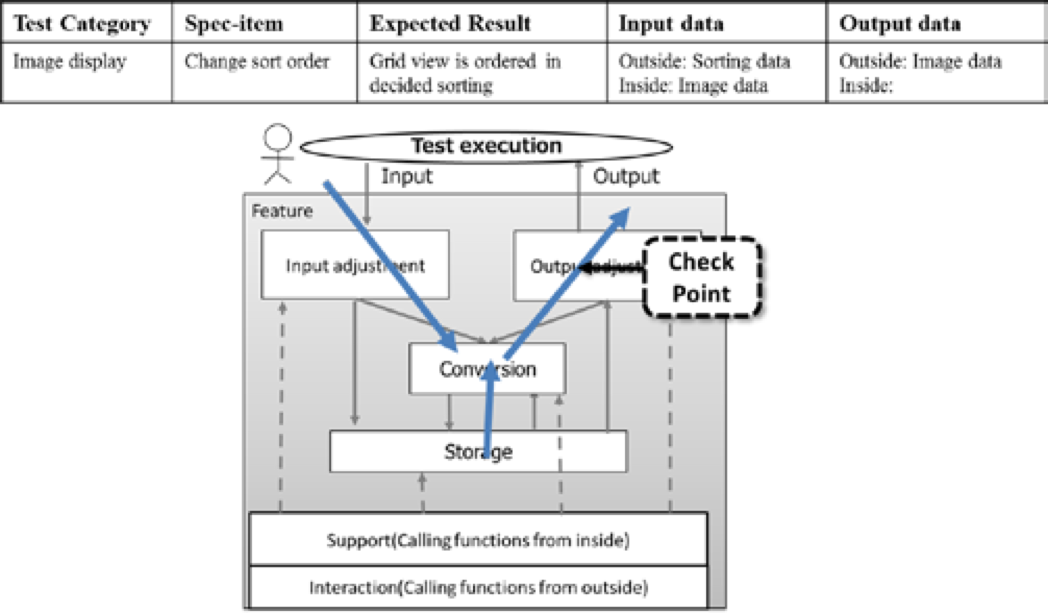
\includegraphics[width=10cm]{./image/D-4-Fig9.png}
\caption{仕様項目に入力データと出力データを加える方法の説明}
\label{fig:D-4-Fig9}
\end{center}
\end{figure}

\end{description}

\subsection{I/Oテストデータパターンを使ったテストベース分析}
I/Oテストデータパターンと既存の分析手法であるテストカテゴリベースドテストを併用してテスト分析を行う.
作業ステップは以下のとおりである:
\begin{itemize}
 \item テストカテゴリを特定する.
 \item テストカテゴリ毎に入力データと出力データを明らかにする
 \item I/Oテストデータパターンごとのデータフローをシミュレーションしてチェックポイント候補から仕様項目を選択する
 \item 現場のテストケースを分析した結果をテストカテゴリに分類し,差異を比較する.
\end{itemize}

特定したテストカテゴリは,表~\ref{tab:D-4-TestCategory}のようになった.
サポートと相互作用については,テストカテゴリがトリガーとなる.トリガーから呼び出す$Ta$へのデータフローをシミュレーションして,仕様項目を特定した.

% Table generated by Excel2LaTeX from sheet 'Sheet2'
\begin{table}[htbp]
  \centering
  \caption{テストカテゴリ}
    \begin{tabular}{|l|l|p{5.415em}|l|l|l|l|}
    \hline
          & \multicolumn{1}{p{3.585em}|}{\textbf{入力調整}} & \textbf{出力調整} & \multicolumn{1}{p{2.5em}|}{\textbf{変換}} & \multicolumn{1}{p{3em}|}{\textbf{貯蔵}} & \multicolumn{1}{p{6em}|}{\textbf{サポート}} & \multicolumn{1}{p{6em}|}{\textbf{相互作用}} \bigstrut\\
    \hline
    \multicolumn{1}{|l|}{\multirow{3}[2]{*}{\textbf{テスト
カテゴリ}}} & \multicolumn{1}{l|}{\multirow{3}[2]{*}{画面上操作}} & 画面表示  & \multicolumn{1}{l|}{\multirow{3}[2]{*}{計算}} & \multicolumn{1}{p{3em}|}{設定保温} & 割り込み  & リソース共有 \bigstrut[t]\\
          &       & メッセージ &       & \multicolumn{1}{p{3em}|}{画像保存} & 中断    & 反映 \\
          &       & 初期表示  &       &       & データ同時変更 & 並列処理 \bigstrut[b]\\
    \hline
    \end{tabular}%
  \label{tab:D-4-TestCategory}%
\end{table}%


\subsection{IOテストデータパターンの効果実証の結果}
テストカテゴリとI/Oテストデータパターンを使ったテストベースの分析で利用したI/Oテストデータパターンは表~\ref{tab:D-4-IOresult}のようになった.
実験に使ったフィーチャセットであるアップロードとグリッドビューの両方でテストカテゴリとI/Oテストデータパターンを使ったテストベースの分析が適用できた.そして,両方のフィーチャセットにて,現実の開発で行われたシステムテストレベルのテストケースとI/Oテストデータパターンを使ったテスト分析結果を比較し,現実の開発で使われたテストケースに,テストすべき仕様項目が不足していることが実証できた.
分類に利用したI/Oテストデータパターンは,P5とP8を除く全てであった.

% Table generated by Excel2LaTeX from sheet 'Sheet3'
\begin{table}[htbp]
  \centering
  \caption{I/Oテストデータパターンの出現傾向}
    \begin{tabular}{|p{7em}|p{1.7em}|p{1.7em}|p{1.7em}|p{1.7em}|p{1.7em}|p{1.7em}|p{1.7em}|p{1.7em}|p{1.7em}|}
    \hline
    \multicolumn{1}{|r|}{} & \multicolumn{1}{l|}{P1} & \multicolumn{1}{l|}{P2} & \multicolumn{1}{l|}{P3} & \multicolumn{1}{l|}{P4} & \multicolumn{1}{l|}{P5} & \multicolumn{1}{l|}{P6} & \multicolumn{1}{l|}{P7} & \multicolumn{1}{l|}{P8} & \multicolumn{1}{l|}{P9} \bigstrut\\
    \hline
    アップロード & ○     & ○     & ○     & ○     & X     & ○     & ○     & X     & ○ \bigstrut\\
    \hline
    グリッドビュー & ○     & X     & X     & ○     & X     & X     & ○     & X     & ○ \bigstrut\\
    \hline
    \end{tabular}%
  \label{tab:D-4-IOresult}%
\end{table}%

実プロジェクトのテスト条件との比較をした結果を図~\ref{fig:D-4-Fig10}に示す.
両者を比較すると,I/Oテストデータパターンを利用したテスト分析の結果が実プロジェクトより多くのテスト条件を選択できたことが確認できている.

\begin{figure}[htbp]
\begin{center}
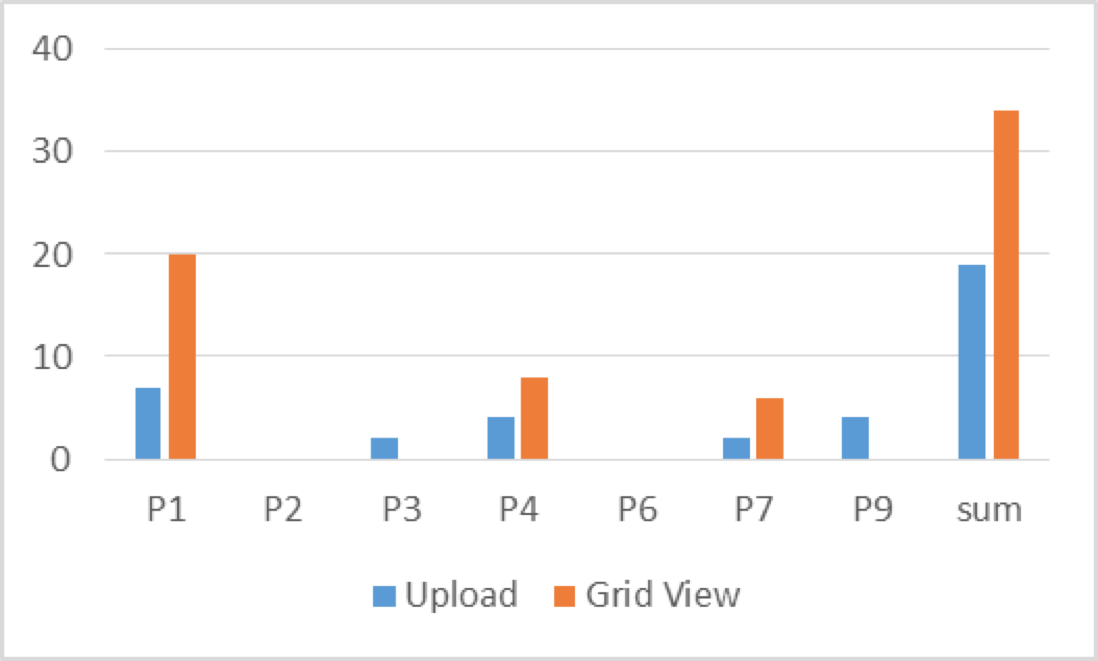
\includegraphics[width=12cm]{./image/D-4-Fig11.png}
\caption{IOテストデータパターンごとの違い}
\label{fig:D-4-Fig10}
\end{center}
\end{figure}

\subsection{I/Oテストデータパターン毎の出現傾向の評価}
現実のプロジェクトで作られたテストケースとI/Oテストデータパターンを使ってテストベースの分析して特定した仕様項目の特定数をP1からP9の分類で出現割合を比較した結果が,表~\ref{tab:D-4-IOtestcompare}である.
% Table generated by Excel2LaTeX from sheet '結果比較'
\begin{table}[htbp]
  \centering
  \caption{I/Oテストデータパターン毎の特定数比較}
    \begin{tabular}{rrrrrrrr}
    \multicolumn{1}{l}{\textbf{アップロード}} &       &       &       &       &       &       &  \bigstrut[b]\\
    \hline
    \multicolumn{1}{|l|}{P1} & \multicolumn{1}{l|}{P2} & \multicolumn{1}{l|}{P3} & \multicolumn{1}{l|}{P4} & \multicolumn{1}{l|}{P6} & \multicolumn{1}{l|}{P7} & \multicolumn{1}{l|}{P9} & \multicolumn{1}{l|}{合計} \bigstrut\\
    \hline
    \multicolumn{1}{|r|}{24} & \multicolumn{1}{r|}{6} & \multicolumn{1}{r|}{12} & \multicolumn{1}{r|}{14} & \multicolumn{1}{r|}{3} & \multicolumn{1}{r|}{7} & \multicolumn{1}{r|}{12} & \multicolumn{1}{r|}{78} \bigstrut\\
    \hline
    \multicolumn{1}{|r|}{17} & \multicolumn{1}{r|}{6} & \multicolumn{1}{r|}{10} & \multicolumn{1}{r|}{10} & \multicolumn{1}{r|}{3} & \multicolumn{1}{r|}{5} & \multicolumn{1}{r|}{8} & \multicolumn{1}{r|}{59} \bigstrut\\
    \hline
    71\%  & 100\% & 83\%  & 71\%  & 100\% & 71\%  & 67\%  & 76\% \bigstrut[t]\\
          &       &       &       &       &       &       &  \\
    \multicolumn{1}{l}{グリッドビュー} &       &       &       &       &       &       &  \bigstrut[b]\\
    \hline
    \multicolumn{1}{|l|}{P1} & \multicolumn{1}{r|}{} & \multicolumn{1}{r|}{} & \multicolumn{1}{l|}{P4} & \multicolumn{1}{r|}{} & \multicolumn{1}{l|}{P7} & \multicolumn{1}{l|}{P9} & \multicolumn{1}{l|}{合計} \bigstrut\\
    \hline
    \multicolumn{1}{|r|}{25} & \multicolumn{1}{r|}{} & \multicolumn{1}{r|}{} & \multicolumn{1}{r|}{13} & \multicolumn{1}{r|}{} & \multicolumn{1}{r|}{14} & \multicolumn{1}{r|}{4} & \multicolumn{1}{r|}{56} \bigstrut\\
    \hline
    \multicolumn{1}{|r|}{5} & \multicolumn{1}{r|}{} & \multicolumn{1}{r|}{} & \multicolumn{1}{r|}{5} & \multicolumn{1}{r|}{} & \multicolumn{1}{r|}{8} & \multicolumn{1}{r|}{4} & \multicolumn{1}{r|}{22} \bigstrut\\
    \hline
    20\%  &       &       & 38\%  &       & 57\%  & 100\% & 39\% \bigstrut[t]\\
    \end{tabular}%
  \label{tab:D-4-IOtestcompare}%
\end{table}%


現実のプロジェクトにて不足していたテスト条件には,I/Oテストデータパターン別にみるとP1が特にテストカテゴリと実プロジェクトの差異が大きいことがわかる.
P1 は外部からの入力を行い,外部に出力する最も単純なパターンであり,I/O テストデータパターンから見ても単純なことを確認するテスト条件が漏れている.

\begin{figure}[htbp]
\begin{center}
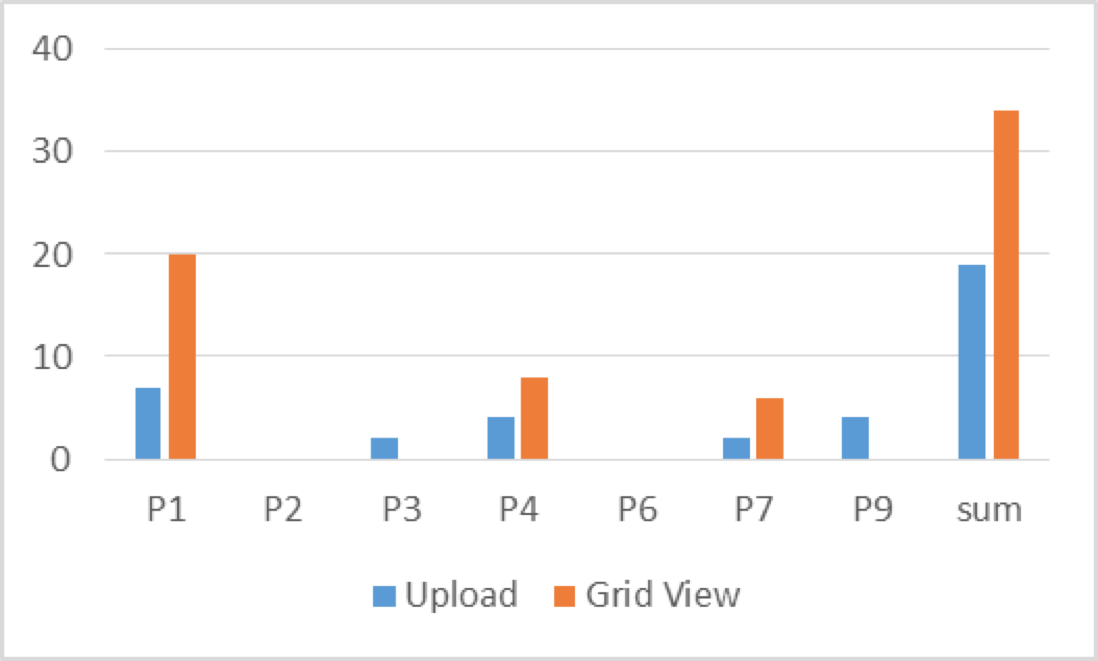
\includegraphics[width=12cm]{./image/D-4-Fig11.png}
\caption{IOテストデータパターンごとの違い}
\label{fig:D-4-Fig11}
\end{center}
\end{figure}

\subsection{現実のプロジェクトにて不足していたテスト条件}
表~\ref{tab:D-4-ER-1}から表~\ref{tab:D-4-ER-4}に,現実のプロジェクトにて不足していたテスト条件となる仕様項目を全て列挙した.これらの仕様項目は,全て今回のデータのI/Oのシミュレーションを行い網羅的にテストベースを確認することで特定できたものである.不足していた仕様項目には,論理的機能構造の要素別に見ると入力調整, 出力調整に分類できる仕様項目,例えばメッセージが現れることや入力制御といった単純な仕様項目でも漏れていることが確認できる.
% Table generated by Excel2LaTeX from sheet 'Sheet2'
\begin{table}[htbp]
  \scriptsize
  \centering
  \caption{現実のプロジェクトにて不足していたテスト条件(1/4)}
    \begin{tabular}{|p{8em}|p{7em}|p{9em}|p{9em}|p{3em}|p{12em}|}
\cline{1-6}   フィーチャーセット & テストカテゴリ  & 仕様項目 & 期待結果  & I/O   & 入出力データ \bigstrut\\
    \hline
    アップロード & データ同時変更 & アップロード中のアップロード済み画像のアルバム移動 & ロックがかかりできないこと & P9    & 外入:画像 内入:移動元画像
外出:件数 内出:画像 \bigstrut\\
    \hline
    アップロード & データ同時変更 & アップロード中のアップロード済み画像の情報変更 & ロックがかかりできないこと & P9    & 外入:情報 内入:画像情報
外出:変情 内出:画像情報 \bigstrut\\
    \hline
    アップロード & データ同時変更 & アップロード中のアップロード先アルバム名変更 & ロックがかかりできないこと & P9    & 外入:画像、アルバム名 内入:元アルバム名
外出:件数 内出:画像 \bigstrut\\
    \hline
    アップロード & データ同時変更 & アップロード中のアップロード前画像のアルバム移動 & ロックがかかりできないこと & P9    & 外入:画像 内入:移動元画像
外出:件数 内出:画像 \bigstrut\\
    \hline
    アップロード & メッセージ & 「画像を選択」時の選択枚数表示 & 「○枚の画像を選択中」というメッセージが出るか & P1    & 外入:画像選択 内入:--
外出:メッセージ 内出:-- \bigstrut\\
    \hline
    アップロード & メッセージ & 重複画像だけでアップロードした際の画像のアップロード & 「アップロードできない」というメッセージがでるか? & P1    & 外入:画像選択 内入:--
外出:メッセージ 内出:-- \bigstrut\\
    \hline
    アップロード & メッセージ & 「画像を選択」画面初期表示 & 「画像を選択」と表記が出ること & P1    & 外入:文字 内入:--
外出:文字 内出:-- \bigstrut\\
    \hline
    アップロード & メッセージ & 「画像を選択」時の選択枚数表示にて、選択済みの画像を押下 & 「○枚の画像を選択」というメッセージの枚数が減ること & P1    & 外入:画像選択 内入:--
外出:メッセージ 内出:-- \bigstrut\\
    \hline
    アップロード & メッセージ & 「画像を選択」時の選択枚数表示にて、選択済みの画像を押下 & 選択数が0になった場合、「画像を選択」と表記が出ること & P1    & 外入:画像選択 内入:--
外出:メッセージ 内出:-- \bigstrut\\
    \hline
    アップロード & 画像表示  & \multicolumn{1}{p{7.5em}|}{「アルバムに追加」でのアルバム一覧} & アルバム一覧の表示順が正しいこと & P4    & 外入:-- 内入:画像サムネイル、アルバム名
外出:画像サムネイル、アルバム名 内出:-- \bigstrut\\
    \hline
    アップロード & 画像表示  & \multicolumn{1}{p{7.5em}|}{「画像を選択」時の画像表示順} & 撮影日昇順で表示されること & p4    & 外入:-- 内入:画像
外出:画像 内出:-- \bigstrut\\
    \hline
    アップロード & 初期表示  & \multicolumn{1}{p{7.5em}|}{「アップロード」画面の操作} & 新規アルバムYYYY/MM/DDというアルバム名が表示されること & P4    & 外入:-- 内入:初期設定
外出:アルバム名 内出:-- \bigstrut\\
    \hline
    アップロード & 初期表示  & \multicolumn{1}{p{7.5em}|}{「アップロード」画面の操作} & 「すでにアップロード済みの画像を保存しない」がONになっていること & P4    & 外入:-- 内入:初期設定
外出:設定 内出:-- \bigstrut\\
    \hline
    アップロード & 画面上操作 & \multicolumn{1}{p{7.5em}|}{「アップロード」画面の操作} & 「すでにアップロード済みの画像を保存しない」がON→OFF→ONに変更できること & P1    & 外入:設定入力 内入:--
外出:設定 内出:-- \bigstrut\\
    \hline
    \end{tabular}%
  \label{tab:D-4-ER-1}%
\end{table}%

% Table generated by Excel2LaTeX from sheet 'Sheet4'
\begin{table}[htbp]

  \scriptsize
  \centering
  \caption{現実のプロジェクトにて不足していたテスト条件(2/4)}
  \begin{tabular}{|p{8em}|p{7em}|p{9em}|p{9em}|p{3em}|p{12em}|}
\cline{1-6}   フィーチャーセット & テストカテゴリ  & 仕様項目 & 期待結果  & I/O   & 入出力データ \bigstrut\\
    \hline
    アップロード & 画面上操作 & \multicolumn{1}{p{7.5em}|}{「アルバムに追加」に表示されるアルバム名} & 「全画像」を選択できること & P7    & 外入:操作入力 内入:登録済画像
外出:登録済画像 内出:-- \bigstrut\\
    \hline
    アップロード & 画面上操作 & 「画像を選択」での画像選択 & 画像にタップするとチェックがつくこと & P7    & 外入:選択 内入:画像
外出:チェックアイコン 内出:-- \bigstrut\\
    \hline
    アップロード & 中断    & \multicolumn{1}{p{7.5em}|}{ネットワーク切断から再開したときのアップロード} & 一定以上の時間が過ぎるとアップロードが再開しない(要確認) & P1    & 外入:画像 内入:--
外出: メッセージ 内出:-- \bigstrut\\
    \hline
    アップロード & 画像保存  & \multicolumn{1}{p{7.5em}|}{アルバムの枚数が200枚以上になる枚数で画像を選択してアップロードのエラーが出た後に別のアルバムを選択してアップロード} & アップロードできた画像がNISにて表示できること & P3    & 外入:画像 内入:--
外出:枚数 内出:画像 \bigstrut\\
    \hline
    アップロード & 画像保存 & \multicolumn{1}{p{7.5em}|}{アップロードした画像の画質} & アップロードした画像が崩れていないこと & P3    & 外入:画像 内入:--
外出:枚数 内出:画像 \bigstrut\\
    \hline
    グリッドビュー & メッセージ & 選択画面初期表示 & 「画像を選択」と表記が出ること & P1    & 入力:文字
出力:文字 \bigstrut\\
    \hline
    グリッドビュー & メッセージ & 選択解除ボタン押下 & 「画像を選択」と表記が出ること & P1    & 入力:選択 文字
出力:文字 \bigstrut\\
    \hline
    グリッドビュー & メッセージ & \multicolumn{1}{p{7.5em}|}{選択済みの画像を押下} & 「○枚の画像を選択」というメッセージの枚数が減ること & P1    & 入力:選択
出力:文字 \bigstrut\\
    \hline
    グリッドビュー & メッセージ & \multicolumn{1}{p{7.5em}|}{選択済みの画像を押下} & 選択数が0になった場合、「画像を選択」と表記が出ること & P1    & 入力:選択
出力:文字 \bigstrut\\
    \hline
    グリッドビュー & メッセージ & 全て選択ボタン押下 & 「アルバムを選択中」というメッセージが出ること & P1    & 入力:選択
出力:文字 \bigstrut\\
    \hline
    グリッドビュー & メッセージ & 未選択の画像を押下 & 「○枚の画像を選択」というメッセージが出ること & P1    & 入力:選択
出力:文字 \bigstrut\\
    \hline
    グリッドビュー & 画像表示  & 1画面あたりの表示ファイル数 & 縦:4×10.横:3×7になること & P4    & 入力:既存設定
出力:文字 画像 \bigstrut\\
    \hline
    \end{tabular}%
  \label{tab:D-4-ER-2}%
\end{table}%

% Table generated by Excel2LaTeX from sheet 'Sheet4'
\begin{table}[htbp]
  \scriptsize
  \centering
  \caption{現実のプロジェクトにて不足していたテスト条件(3/4)}
  \begin{tabular}{|p{8em}|p{7em}|p{9em}|p{9em}|p{3em}|p{12em}|}
\cline{1-6}   フィーチャーセット & テストカテゴリ  & 仕様項目 & 期待結果  & I/O   & 入出力データ \bigstrut\\
    \hline
    グリッドビュー & 画像表示  & スクロール時の枚数表示 & 複数ページのスクロールでファイルの日付と、現在の枚数順/全体の枚数が画面中央に表示されること & p7    & 入力:スクロール
出力:文字 画像 \bigstrut\\
    \hline
    グリッドビュー & 画像表示  & 画像ファイルの並び順 & 左から右方向に埋まっていくこと。 & P4    & 入力:既存設定
出力:文字 画像 \bigstrut\\
    \hline
    グリッドビュー & 画像表示  & 画像ファイルの並び順 & 2行目になるとまた左から埋まること & P4    & 入力:既存設定
出力:文字 画像 \bigstrut\\
    \hline
    グリッドビュー & 画像表示  & 更新ボタン押下 & 別デバイスで新しい画像の追加、名称の変更などをしていた場合、変更した画像に更新されること & P4    & 入力:既存設定
出力:画像 \bigstrut\\
    \hline
    グリッドビュー & 共有    & 他ビューの並び順影響有無 & 他のアルバムやビューで設定した並び順の影響を受けないこと & p4    & 入力:既存設定
出力:画像 \bigstrut\\
    \hline
    グリッドビュー & 設定保存  & 画面の並び順設定用画面 & 前回選択した並び順にチェックがついていること & p7    & 入力:並び順
出力:並び順 \bigstrut\\
    \hline
    グリッドビュー & 設定保存  & 画面の並び順設定用画面 & デフォルトでチェックされていること & p7    & 入力:並び順
出力:並び順 \bigstrut\\
    \hline
    グリッドビュー & 画面上操作 & OKボタン押下 & 全画像,カテゴリから移動したグリッドビューの場合のみOKボタンが現れ、共有設定画面に遷移する & P1    & 入力:既存設定
出力:画像 \bigstrut\\
    \hline
    グリッドビュー & 画面上操作 & \multicolumn{1}{p{7.5em}|}{アルバム追加ボタン押下} & アルバムから移動したグリッドビューの場合,アルバム追加画面に遷移する & P1    & 入力:既存設定
出力:文字 画像 \bigstrut\\
    \hline
    グリッドビュー & 画面上操作 & ダウンロードボタン押下 & アルバムから移動したグリッドビューの場合,DLサイズ選択画面に遷移する & P1    & 入力:既存設定
出力:文字 \bigstrut\\
    \hline
    グリッドビュー & 画面上操作 & 削除ボタン押下 & アルバムから移動したグリッドビューの場合,削除画面に遷移 & P1    & 入力:既存設定
出力:文字 \bigstrut\\
    \hline
    \multicolumn{1}{|l|}{グリッドビュー} & 画面上操作 & 選択画面初期表示 & 全画像から遷移したグリッドビューの場合,選択,解除,削除、アルバム追加、DLボタン出ない.OKボタン出る. & P1    & 入力:既存設定
出力:文字 画像 \bigstrut\\
    \hline
    \multicolumn{1}{|l|}{グリッドビュー} & 画面上操作 & 選択画面初期表示 & カテゴリから遷移したグリッドビューの場合、全画像からの遷移と同じであり,かつカテゴリを選択する選択用ビューがグレーアウトする & P1    & 入力:既存設定
出力:文字 画像 \bigstrut\\
    \hline
    \end{tabular}%
  \label{tab:D-4-ER-3}%
\end{table}%

% Table generated by Excel2LaTeX from sheet 'Sheet4'
    \begin{table}[htbp]
      \scriptsize
      \centering
      \caption{現実のプロジェクトにて不足していたテスト条件(4/4)}
      \begin{tabular}{|p{8em}|p{7em}|p{9em}|p{9em}|p{3em}|p{12em}|}
    \cline{1-6}   フィーチャーセット & テストカテゴリ  & 仕様項目 & 期待結果  & I/O   & 入出力データ \bigstrut\\
        \hline
    \multicolumn{1}{|l|}{グリッドビュー} & 画面上操作 & 選択画面初期表示 & 端末の写真のグリッドビューの場合、最初から選択画面となり、チェックをすることでOKボタンが有効になる & P1    & 入力:既存設定
出力:文字 画像 \bigstrut\\
    \hline
    \multicolumn{1}{|l|}{グリッドビュー} & 画面上操作 & 選択解除ボタン押下 & 画面上の全ての画像のチェックが外れること & p1    & 入力:選択
出力:アイコン \bigstrut\\
    \hline
    \multicolumn{1}{|l|}{グリッドビュー} & 画面上操作 & \multicolumn{1}{p{7.5em}|}{選択済みの画像を押下} & 画像のチェックが外れること & p1    & 入力:選択
出力:アイコン \bigstrut\\
    \hline
    \multicolumn{1}{|l|}{グリッドビュー} & 画面上操作 & 全て選択ボタン押下 & 画面上の全ての画像にチェックがつくこと & p1    & 入力:選択
出力:アイコン \bigstrut\\
    \hline
    \multicolumn{1}{|l|}{グリッドビュー} & 画面上操作 & 未選択の画像を押下 & 画像のチェックがつくこと & p1    & 入力:選択
出力:アイコン \bigstrut\\
    \hline
    \multicolumn{1}{|l|}{グリッドビュー} & 画面上操作 & 未選択の画像を押下 & 全てチェックの場合、押下した画像以外のチェックが全て外れること & p1    & 入力:選択
出力:アイコン \bigstrut\\
    \hline
    \multicolumn{1}{|l|}{グリッドビュー} & 画面上操作 & フロービューボタン押下 & フロービューに遷移すること & P7    & 入力:既存設定
出力:文字 画像 \bigstrut\\
    \hline
    \multicolumn{1}{|l|}{グリッドビュー} & 画面上操作 & マップビュー押下 & マップビューに遷移すること & P7    & 入力:既存設定
出力:文字 画像 \bigstrut\\
    \hline
    \multicolumn{1}{|l|}{グリッドビュー} & 画面上操作 & 画像選択ボタン押下 & ピクチャービューに遷移すること & P7    & 入力:既存設定
出力:文字 画像 \bigstrut\\
    \hline
    \multicolumn{1}{|l|}{グリッドビュー} & 画面上操作 & 画面の並び順設定用画面 & ファイル名、アップロード名、撮影日、ファイルサイズ、ファイル形式、お気に入り、マイルールの順で一覧表示されていること & P1    & 入力:既存設定
出力:文字 \bigstrut\\
    \hline
    \multicolumn{1}{|l|}{グリッドビュー} & 画面上操作 & 並び順の変更 & 一覧項目の横をタップするとチェックがつくこと & p1    & 入力:設定
出力:設定 \bigstrut\\
    \hline
    グリッドビュー & 中断    & ネットワーク切断時のグリッドビュー初期表示 & キャッシュがある場合、キャッシュされた画像が一覧表示されること & P4    & 入力:既存設定
出力:文字 画像 \bigstrut\\
    \hline
    グリッドビュー & 中断    & ネットワーク切断時のグリッドビュー初期表示 & キャッシュの限界を超えた場合、その画像が一覧表示されないこと & P4    & 入力:既存設定
出力:文字 画像 \bigstrut\\
    \hline
    グリッドビュー & 中断    & ネットワーク切断時の更新ボタン押下 & キャッシュがある場合、更新ボタンを押すと別デバイスの変更が反映されず画像が表示される & P4    & 入力:既存設定
出力:文字 画像 \bigstrut\\
    \hline
    \end{tabular}%
    \label{tab:D-4-ER-4}%
  \end{table}%

一般的に,テスト条件となる仕様項目の一覧を作成せずに具体的なインスタンスとなるテストケースを列挙していく場合,テストパラメータ組み合わせの数量の多さに合わせてテストケースの数量が膨大になるため,網羅すべきテスト条件仕様項目の見易さが低下するため,仕様項目の数が不足することが多い.
実験結果も同様の傾向となった.

\newpage
\section{まとめ}
 本論文では,テスト実行時のデータI/Oの要素で分類し網羅的に分析する方法を提案した.そして,現場のテストプロジェクトのテストケースを使い,提案した方法の実証を試みた.結果的に,提案した方法で特定した仕様項目と実プロジェクトで作られるテストケースと比較して,不足している仕様項目の発見が可能であることが確認できた.
